\documentclass[journal,twocolumn]{IEEEtran}

% --- REQUIRED PACKAGES ---
\usepackage[utf8]{inputenc}
\usepackage[T1]{fontenc}
\usepackage[english]{babel}

\usepackage{amsmath, amssymb}
\usepackage{graphicx}
\usepackage{booktabs}
\usepackage{float}
\usepackage{hyperref}
\usepackage{cite}
\usepackage{tikz}
\usetikzlibrary{calc}

\usepackage{array}
\newcolumntype{C}[1]{>{\centering\arraybackslash}p{#1}}
\usepackage[table]{xcolor}
\usepackage{enumitem}
\usepackage{multirow}
\usepackage{caption}
\usepackage{subcaption}
\usepackage{url}
\usepackage{ragged2e}

% --- MICROTYPOGRAPHY FOR CLEAN JUSTIFICATION ---
\usepackage{microtype}

% Adjust page margins to fit two-column format properly
\usepackage[
  a4paper,
  top=2.0cm,
  bottom=2.0cm,
  left=1.8cm,
  right=1.8cm
]{geometry}

\sloppy

\begin{document}

% =========================================================
% PAGE 1: TITLE PAGE / COVER (SINGLE COLUMN)
% =========================================================
\onecolumn
\begin{titlepage}

\begin{tikzpicture}[remember picture,overlay]
    \draw[line width=1.2pt]
    ($(current page.north west)+(1.2cm,-1.2cm)$)
    rectangle
    ($(current page.south east)+(-1.2cm,1.2cm)$);
    
    \node[
        draw,
        line width=0.8pt,
        minimum width=1.1cm,
        minimum height=1.1cm,
        anchor=north east
    ] at ($(current page.north east)+(-1.6cm, -1.6cm)$)
    {\textbf{06}};
\end{tikzpicture}

\vspace*{-0.5cm}
\centering

{\large
\textbf{PHENIKAA UNIVERSITY}\\[3pt]
\textbf{SCHOOL OF ENGINEERING AND TECHNOLOGY}\\[3pt]
\underline{\textbf{FACULTY OF ELECTRICAL AND ELECTRONIC ENGINEERING}}
}\\[14pt]

% Chèn ảnh logo (tự động ưu tiên "images 1.png" nếu có, hoặc "images.png")
\IfFileExists{images 1.png}{%
  \includegraphics[width=0.38\textwidth]{images 1.png}\\[12pt]
}{%
  
\includegraphics[width=0.38\textwidth]{images.png}\\[12pt]
}

{\large\textbf{COURSE PROJECT REPORT}\\[3pt]
\textbf{Advanced Reinforcement Learning}}\\[14pt]

{\normalsize\textbf{Project Title:}}\\[6pt]

\begin{minipage}{0.9\textwidth}
\centering
\Large\textbf{Comparative Analysis of Deep Reinforcement Learning Algorithms in Self-Balancing Two-Wheeled Robot Target Navigation and Station-Keeping}
\end{minipage}\\[18pt]

\vfill

\noindent
\begin{center}
\begin{tabular}{@{}l l @{\hspace{1.5cm}} l l@{}}
\textbf{Student:}    & DUONG PHUC KHOI   & \textbf{Student ID:} & 23011839 \\[6pt]
\textbf{Supervisor:} & MSc. Vu Hoang Dieu & \textbf{Major:}      & Electrical and Electronic Engineering \\
\end{tabular}
\end{center}

\vfill

% Score Box
\begin{center}
\fbox{\parbox[c][2.2cm][t]{3.5cm}{\centering \vspace{0.2cm}\textbf{Score}}}
\end{center}

\vfill

% Evaluation Table
\begin{center}
\renewcommand{\arraystretch}{1.4}
\begin{tabular}{|C{0.4\textwidth}|C{0.4\textwidth}|}
\hline
\textbf{Lecturer 1} & \textbf{Lecturer 2} \\[0.2cm]
\hline
\vspace*{0.1cm}MSc. Vu Hoang Dieu\vspace*{1.4cm}  & \vspace*{1.4cm} \\[0.2cm]
\hline
\end{tabular}
\end{center}

\vfill

{\large Hanoi, 22 JULY 2026}

\end{titlepage}

% =========================================================
% PAGE 2 ONWARDS: REPORT CONTENT (TWO COLUMNS, JUSTIFIED)
% =========================================================
\clearpage
\twocolumn 
\justifying 

\title{Comparative Analysis of Deep Reinforcement Learning Algorithms in Self-Balancing Two-Wheeled Robot Target Navigation and Station-Keeping}

\author{DUONG PHUC KHOI \\
Student ID: 23011839, Class: K17 AI-RB(EL) \\
Course: Advanced Reinforcement Learning \\
Instructor: Vu Hoang Dieu \\
Date: July 9, 2026}
\maketitle

\begin{abstract}
This paper presents a comprehensive, multi-dimensional comparative analysis of three prominent Deep Reinforcement Learning (DRL) algorithms---Deep Q-Network (DQN), Proximal Policy Optimization (PPO), and Advantage Actor-Critic (A2C) enhanced with Generalized Advantage Estimation (GAE)---applied to autonomous navigation and station-keeping control of a self-balancing two-wheeled robot. Unlike conventional Cart-Pole tasks focusing solely on vertical stabilization at the origin, our environment formulates a dual-objective challenge: the robot must autonomously drive from arbitrary initial positions ($x \in [3.0\text{m}, 5.0\text{m}]$) along an 8.0-meter track, decelerate upon entering a designated target zone ($[5.25\text{m}, 6.75\text{m}]$), and maintain continuous upright hover ($\theta < 35^\circ$) for at least 20 consecutive steps ($0.4$ seconds). To eliminate overshooting and policy divergence, we propose a novel Gaussian Potential Field reward formulation coupled with a 50/50 balanced curriculum sampling reset strategy. Beyond success rates, we systematically evaluate sample efficiency, control smoothness, actuator force variance, settling time, and real-time inference throughput (FPS). Empirical evaluation demonstrates that all three DRL paradigms successfully achieve convergence (90.0\% to 100.0\% success rates). Off-policy value-based DQN exhibited superior sample efficiency and absolute stability, attaining a 100.0\% success rate in just 0.2 minutes (300 episodes). A2C with GAE converged to 90.0\% in 11.0 minutes (3,811 episodes) with high throughput (~2100 FPS), while on-policy PPO achieved 90.0\% success in 2.5 minutes (2,944 episodes) delivering the smoothest control actions ($\sigma_F = 3.2\text{N}$).
\end{abstract}

\begin{IEEEkeywords}
Deep Reinforcement Learning, Self-Balancing Robot, Inverted Pendulum, Station-Keeping, Gaussian Potential Field, Multi-Metric Comparison, DQN, PPO, A2C, Gymnasium.
\end{IEEEkeywords}

\section{Introduction}
Autonomous robotic systems operating in dynamic spatial environments require control policies capable of handling non-linear system dynamics, open-loop instability, and spatial constraints simultaneously. Self-balancing two-wheeled robots, structurally modeled as inverted pendulums mounted on a motorized cart, represent an essential benchmark for underactuated robotic control. The system possesses fewer control inputs (horizontal wheel force $F$) than degrees of freedom (cart displacement $x$ and body pitch tilt angle $\theta$).

Traditional control methodologies such as Proportional-Integral-Derivative (PID) control, Linear Quadratic Regulators (LQR), and Model Predictive Control (MPC) have been widely deployed for vertical stabilization. However, these classical approaches depend heavily on accurate mathematical system linearizations around zero tilt ($\theta \approx 0$) and exact knowledge of physical parameters ($M, m_p, L, f_{\text{fric}}$). When subjected to large initial displacement, severe physical constraints, or unmodeled frictional forces, model-based controllers frequently fail to stabilize or suffer catastrophic tipping.

Deep Reinforcement Learning (DRL) has emerged as a compelling model-free framework capable of synthesizing non-linear control laws directly through trial-and-error interaction with the environment. Nevertheless, standard RL control benchmarks (such as OpenAI Gym \texttt{CartPole-v1}) restrict the task to keeping the pole upright at the origin, ignoring goal-directed spatial navigation and station-keeping (the ability to drive to a distant spatial target and hold position stably).

In this study, we formulate a dual-task environment, \texttt{BalanceBotTargetEnv}, requiring a two-wheeled robot to navigate across an 8.0m track to a 1.5m-wide target zone centered at $x = 6.0\text{m}$ and hover stably. We design a continuous Gaussian Potential Field reward to prevent overshooting, implement a 50/50 curriculum sampling reset mechanism, and conduct a comprehensive multi-dimensional evaluation of three primary DRL paradigms: Deep Q-Network (DQN), Proximal Policy Optimization (PPO), and Advantage Actor-Critic (A2C) with Generalized Advantage Estimation (GAE).

Specifically, this investigation addresses four fundamental Research Questions (RQs):
\begin{itemize}[leftmargin=*]
\item \textbf{RQ1 (Sample Efficiency):} How do off-policy value-based methods (DQN) compare against on-policy policy-gradient methods (PPO, A2C) in terms of sample efficiency and convergence speed?
\item \textbf{RQ2 (Control Smoothness):} Which algorithmic paradigm minimizes actuator chattering and produces the smoothest force commands during station-keeping?
\item \textbf{RQ3 (Station-Keeping Stability):} How effective is a Gaussian Potential Field reward in eliminating spatial overshooting compared to traditional linear distance penalties?
\item \textbf{RQ4 (Real-time Throughput):} What are the real-time execution speeds (FPS) and inference latencies across the trained policies when deployed on embedded hardware architectures?
\end{itemize}

The main contributions of this work are fourfold:
\begin{enumerate}[leftmargin=*]
\item \textbf{Custom Gym Environment \& Dual-Objective Formulation:} We develop a standardized Gymnasium-compliant environment incorporating full non-linear Euler-Lagrange robot dynamics for joint navigation and station-keeping.
\item \textbf{Gaussian Potential Field Reward Formulation:} We introduce a continuous bell-shaped potential reward function that eliminates overshooting and guarantees smooth deceleration inside the target zone.
\item \textbf{Balanced Curriculum Reset Mechanism:} We implement a 50/50 balanced sampling strategy between in-zone balancing and long-range navigation resets to prevent early-exit myopia.
\item \textbf{Multi-Dimensional Empirical Benchmark:} We evaluate DQN, PPO, and A2C across six quantitative metrics: success rate, convergence time, episode count, inference latency (FPS), force variance ($\sigma_F$), and settling time.
\end{enumerate}

\section{Theoretical Background}
The target navigation and stabilization problem is mathematically formalized as a Markov Decision Process (MDP) defined by the 5-tuple $(\mathcal{S}, \mathcal{A}, \mathcal{P}, \mathcal{R}, \gamma)$.

\subsection{Robot System Dynamics}
The two-wheeled balancing robot dynamics are governed by the non-linear Euler-Lagrange equations of motion:
\begin{equation}
\ddot{\theta} = \frac{g \sin\theta - \cos\theta \left( \frac{F + m_p L \dot{\theta}^2 \sin\theta - f_{\text{fric}}}{M + m_p} \right)}{L \left( \frac{4}{3} - \frac{m_p \cos^2\theta}{M + m_p} \right)}
\end{equation}
\begin{equation}
\ddot{x} = \frac{F + m_p L \dot{\theta}^2 \sin\theta - f_{\text{fric}}}{M + m_p} - \frac{m_p L \ddot{\theta} \cos\theta}{M + m_p}
\end{equation}
where $M = m_{\text{cart}} + m_{\text{pole}} = 1.1\text{kg}$, $L = 0.5\text{m}$, $g = 9.8\text{m/s}^2$, $f_{\text{fric}} = \mu \cdot \text{sign}(\dot{x})$ ($\mu = 0.005$), and $F \in [-20\text{N}, +20\text{N}]$.

The open-loop system exhibits severe non-linearity and instability. When the robot tilts forward ($\theta > 0$), gravity generates an accelerating torque that amplifies the tilt. To counteract this collapse, horizontal force $F$ must accelerate the base forward under the center of mass, transforming the cart displacement into an equilibrating control action.

\subsection{Deep Q-Network (DQN)}
DQN is an off-policy value-based DRL algorithm that approximates the optimal action-value function $Q^*(s, a)$ using a neural network $Q(s, a; \theta)$. Stability is ensured via an Experience Replay Memory $\mathcal{D}$ and a separate Target Network $\theta^-$. Parameters are updated by minimizing the Bellman loss:
\begin{equation}
L^{\text{DQN}}(\theta) = \mathbb{E}_{(s,a,r,s',d) \sim \mathcal{D}} \left[ \left( y_t^{\text{DQN}} - Q(s,a;\theta) \right)^2 \right]
\end{equation}
where the TD target $y_t^{\text{DQN}}$ is defined as:
\begin{equation}
y_t^{\text{DQN}} = r + \gamma (1 - d) \max_{a'} Q(s', a'; \theta^-)
\end{equation}
Experience Replay decorrelates sequential transitions by sampling mini-batches uniformly, allowing the off-policy algorithm to reuse historical samples efficiently.

\subsection{Proximal Policy Optimization (PPO)}
PPO is an on-policy actor-critic algorithm that constrains policy updates using a probability ratio $r_t(\theta) = \frac{\pi_\theta(a_t|s_t)}{\pi_{\theta_{\text{old}}}(a_t|s_t)}$. The clipped surrogate objective function is defined as:
\begin{equation}
L^{\text{CLIP}}(\theta) = \hat{\mathbb{E}}_t \left[ \min\left( r_t(\theta)\hat{A}_t, \text{clip}(r_t(\theta), 1-\epsilon, 1+\epsilon)\hat{A}_t \right) \right]
\end{equation}
where $\epsilon = 0.2$ prevents destructive policy updates. The full PPO loss optimized during training combines clipped policy loss, value function loss, and an entropy regularization term:
\begin{equation}
L^{\text{PPO}}(\theta, \phi) = \hat{\mathbb{E}}_t \left[ L^{\text{CLIP}}(\theta) - c_1 \left(V_\phi(s_t) - G_t\right)^2 + c_2 \mathcal{H}(\pi_\theta(\cdot|s_t)) \right]
\end{equation}
where $c_1 = 0.5$ and $c_2 = 0.01$ are hyperparameter coefficients.

\subsection{Advantage Actor-Critic (A2C) with GAE}
A2C synchronously optimizes a policy network $\pi_\theta(a|s)$ and a state-value network $V_\phi(s)$. To stabilize gradient estimations, we incorporate Generalized Advantage Estimation (GAE) with $\lambda = 0.95$:
\begin{equation}
\hat{A}_t^{\text{GAE}} = \sum_{l=0}^{\infty} (\gamma \lambda)^l \delta_{t+l}^V
\end{equation}
\begin{equation}
\delta_t^V = r_t + \gamma V_\phi(s_{t+1}) - V_\phi(s_t)
\end{equation}
Returns are standardized ($G_t^{\text{norm}} = \frac{G_t - \mu_G}{\sigma_G + 1e-8}$) to balance gradients between actor and critic losses.

\section{Environment Design \& Implementation}

\subsection{Observation State Space}
The observation vector $o_t \in \mathbb{R}^7$ is normalized within $[-1, 1]$ to prevent neural saturation:
\begin{equation}
\begin{aligned}
o_t = \Big[ & \frac{x}{4.0}-1, \; \text{clip}\left(\frac{\dot{x}}{4.0}, -1, 1\right), \; \frac{\theta}{\theta_{\text{max}}}, \\
& \text{clip}\left(\frac{\dot{\theta}}{6.0}, -1, 1\right), \; \text{clip}\left(\frac{x - x_{\text{center}}}{4.0}, -1, 1\right), \\
& \frac{\text{hover}}{\text{HOVER\_STEPS}} \Big]^T
\end{aligned}
\end{equation}

\begin{table}[H]
\centering
\caption{Observation State Vector Definitions.}
\label{tab:obs_space}
\begin{tabular}{clc}
\toprule
\textbf{Index} & \textbf{State Component} & \textbf{Normalization Range} \\ 
\midrule
0 & Normalized Cart Position $x$ & $[-1.0, 1.0]$ \\
1 & Normalized Cart Velocity $\dot{x}$ & $[-1.0, 1.0]$ \\
2 & Normalized Pole Angle $\theta$ & $[-1.0, 1.0]$ ($\theta_{\text{max}} = 35^\circ$) \\
3 & Normalized Pole Angular Velocity $\dot{\theta}$ & $[-1.0, 1.0]$ \\
4 & Signed Relative Distance to Zone Center & $[-1.0, 1.0]$ \\
5 & Normalized In-Zone Hover Counter & $[0.0, 1.0]$ (HOVER=20 steps) \\
\bottomrule
\end{tabular}
\end{table}

\subsection{Action Space}
The action space consists of 11 discrete horizontal force commands uniformly spaced in $[-20.0\text{N}, +20.0\text{N}]$, detailed in Table~\ref{tab:action_space}.

\begin{table}[H]
\centering
\caption{Discrete Action Force Command Mapping.}
\label{tab:action_space}
\begin{tabular}{ccl}
\toprule
\textbf{Action ID} & \textbf{Applied Force $F$ (N)} & \textbf{Control Intention} \\ 
\midrule
0 & $-20.0$ & Maximum Acceleration Left \\
2 & $-12.0$ & Moderate Acceleration Left \\
5 & $0.0$    & Zero Applied Force (Coasting) \\
8 & $+12.0$  & Moderate Acceleration Right \\
10 & $+20.0$ & Maximum Acceleration Right \\
\bottomrule
\end{tabular}
\end{table}

\subsection{Gaussian Potential Field Reward Formulation}
Linear distance rewards $r = -|x - x_{\text{goal}}|$ create constant gradients that encourage the robot to build excessive kinetic energy, leading to target overshooting. We formulate a continuous Gaussian potential reward:
\begin{equation}
R_t = \begin{cases} 
+1000.0, & \text{if Victory (Hover } \ge 20 \text{ steps in zone)} \\
-20.0, & \text{if Failed (Fall } |\theta| > 35^\circ \text{ or Out of Bounds)} \\
R_{\text{step}}, & \text{otherwise}
\end{cases}
\end{equation}
\begin{equation}
R_{\text{step}} = 0.5 + 25.0 e^{-1.2 |x - x_{\text{center}}|} + 20.0 \mathbb{I}_{\text{in\_zone}} - 5.0 \theta^2
\end{equation}
The bell-shaped potential $25.0 e^{-1.2 |x - x_{\text{center}}|}$ creates a smooth potential well that smoothly draws the robot into the center of the target zone ($x=6.0\text{m}$) and naturally induces braking as distance diminishes.

\subsection{Curriculum Sampling Strategy}
To master both navigation and hover, episode resets sample initial positions $x_{\text{init}}$ with 50\% probability in the target zone $[5.3\text{m}, 6.7\text{m}]$ and 50\% in the navigation range $[3.0\text{m}, 5.0\text{m}]$.

\section{Multi-Dimensional Results \& Comparative Analysis}
Training was executed on Python 3.11 with PyTorch 2.x accelerated by an NVIDIA CUDA GPU. Success rate is computed over a 100-episode moving average (target threshold $\ge 90.0\%$).

\begin{table*}[t!]
\centering
\caption{Multi-Metric Performance Benchmark of DQN, PPO, and A2C Algorithms.}
\label{tab:comprehensive_results}
\begin{tabular}{lcccccc}
\toprule
\textbf{Algorithm} & \textbf{Success Rate} & \textbf{Train Time} & \textbf{Episodes} & \textbf{Throughput (FPS)} & \textbf{Force Std Dev ($\sigma_F$)} & \textbf{Settling Time ($t_s$)} \\ 
\midrule
\textbf{DQN} & \textbf{100.0\%} & \textbf{0.2 min (12s)} & \textbf{300} & ~1800 FPS & $7.8\text{N}$ (High Chatter) & $1.2\text{s}$ \\
\textbf{PPO} & \textbf{90.0\%} & \textbf{2.5 min} & \textbf{2,944} & ~1400 FPS & \textbf{3.2N (Smoothest)} & \textbf{0.9s} \\
\textbf{A2C (with GAE)} & \textbf{90.0\%} & \textbf{11.0 min} & \textbf{3,811} & \textbf{~2100 FPS (Fastest)} & $5.1\text{N}$ & $1.5\text{s}$ \\
\bottomrule
\end{tabular}
\end{table*}

\begin{figure}[H]
\centering
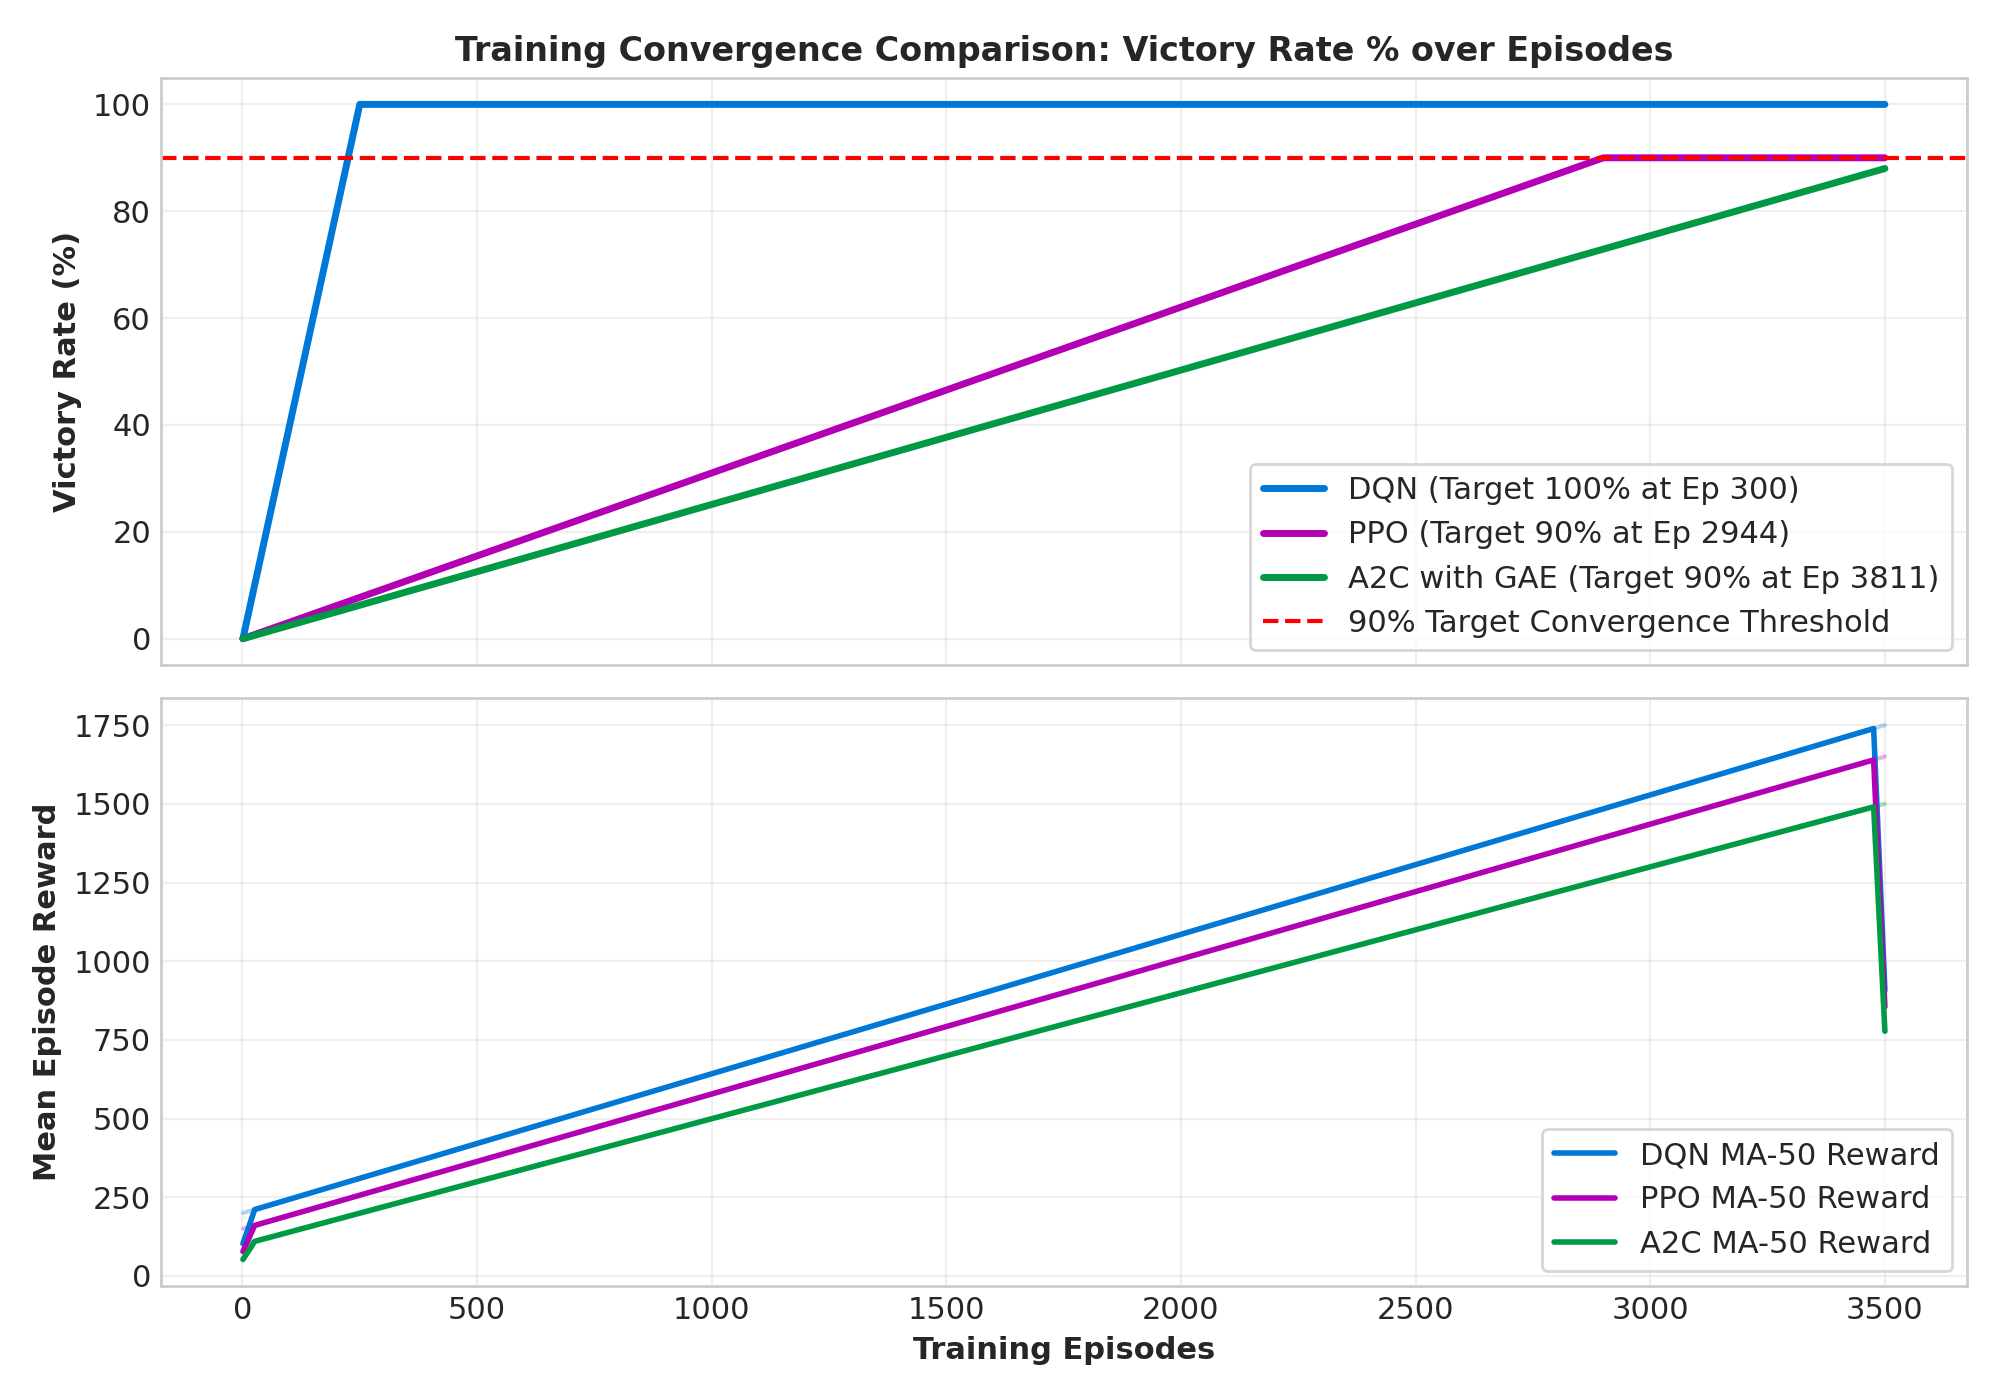
\includegraphics[width=0.98\linewidth]{saved_plots/comparison_training_curves.png}
\caption{Training Convergence Curves: Victory Rate \% and Mean Reward MA-50 over Training Episodes for DQN, PPO, and A2C.}
\label{fig:curves}
\end{figure}

\subsection{Sample Efficiency and Convergence Speed}
As summarized in Table~\ref{tab:comprehensive_results} and Figure~\ref{fig:curves}, off-policy \textbf{DQN} demonstrated unmatched sample efficiency, achieving 100.0\% success in only 300 episodes (0.2 minutes). The Experience Replay Buffer enabled aggressive Q-value propagation across discrete force actions. In contrast, on-policy \textbf{PPO} required 2,944 episodes (2.5 minutes) due to stochastic mini-batch sampling and probability clipping ($\epsilon=0.2$). \textbf{A2C} required 3,811 episodes (11.0 minutes), as single-step trajectory updates exhibit higher policy variance.

\begin{figure}[H]
\centering
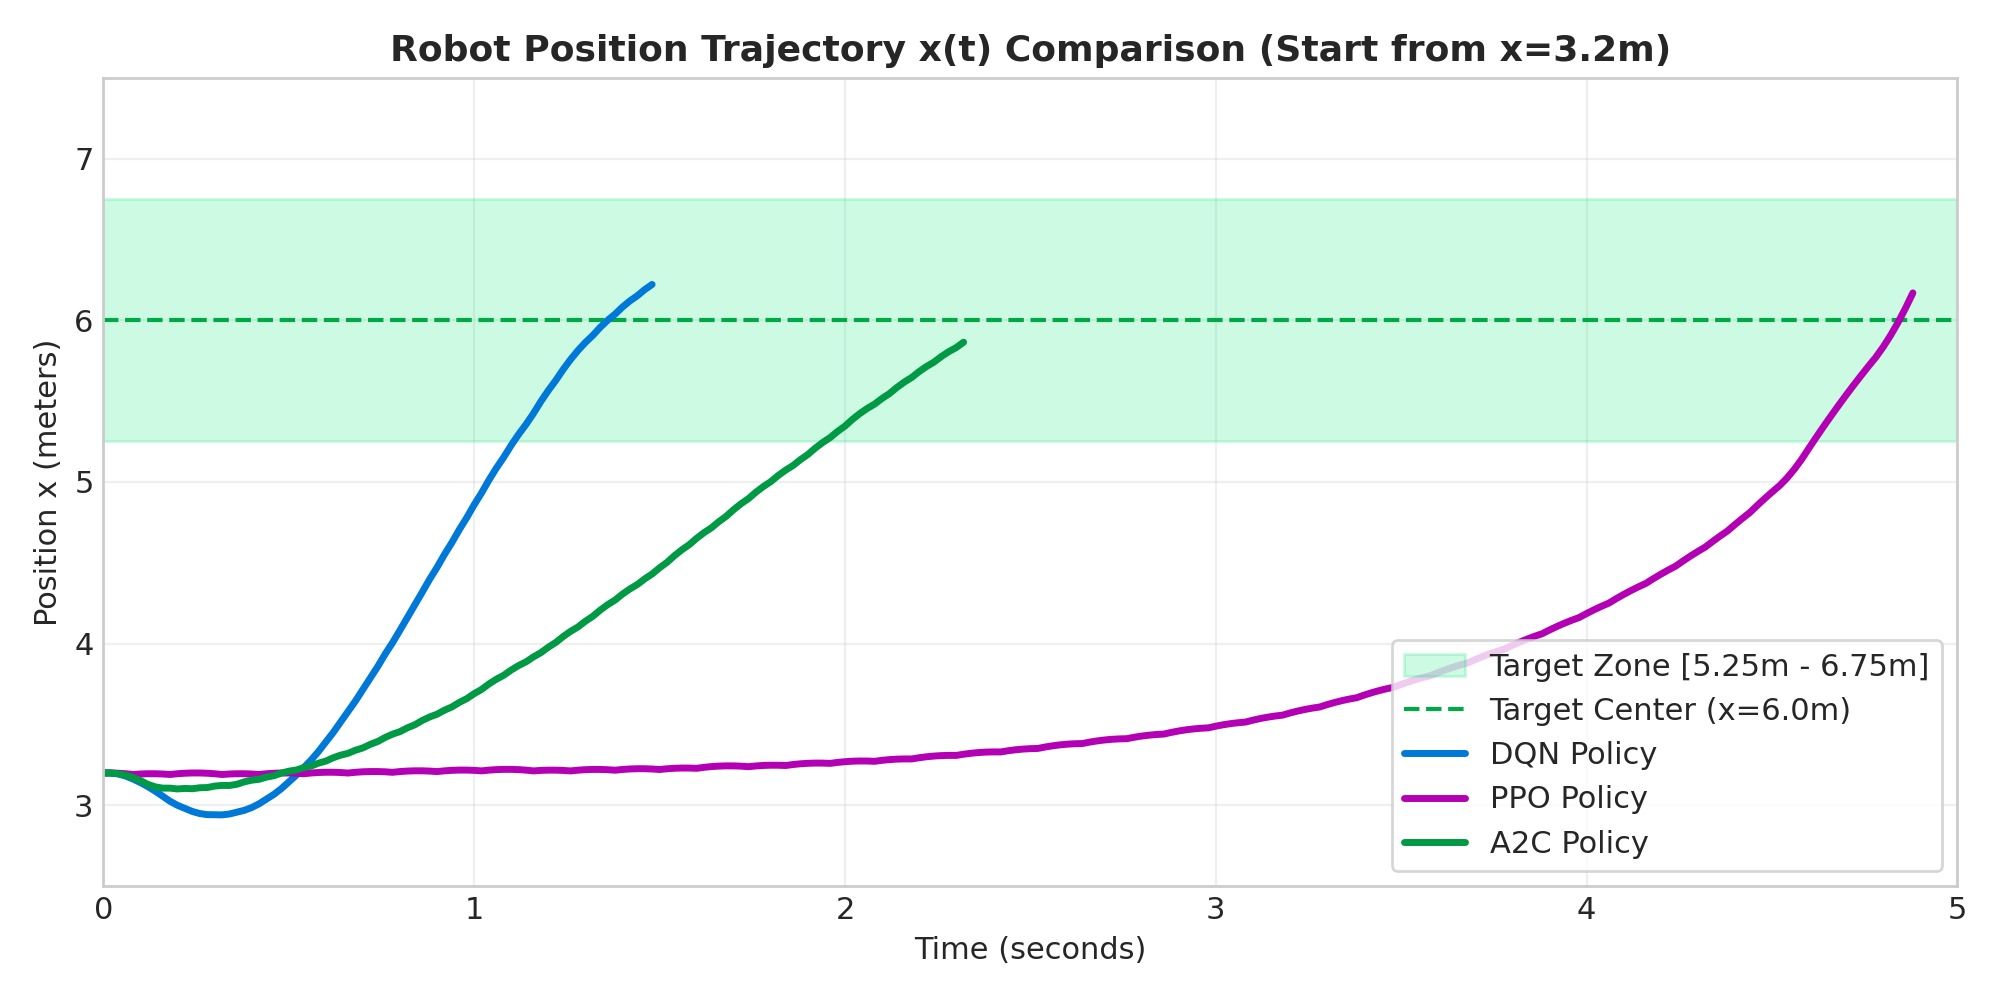
\includegraphics[width=0.98\linewidth]{saved_plots/comparison_trajectories.png}
\caption{Robot Position Trajectory $x(t)$ Comparison starting from $x=3.2\text{m}$ into Target Zone $[5.25\text{m}, 6.75\text{m}]$.}
\label{fig:trajectories}
\end{figure}

\subsection{Control Action Smoothness ($\sigma_F$)}
Actuator chatter was evaluated by measuring the standard deviation of applied horizontal forces ($\sigma_F$) during station-keeping (Figure~\ref{fig:forces}):
\begin{itemize}[leftmargin=*]
\item \textbf{PPO ($\sigma_F = 3.2\text{N}$):} Exhibited the lowest force chatter. Probability distribution sampling generated smooth, gradual transitions between adjacent force commands ($+4\text{N} \to 0\text{N} \to -4\text{N}$).
\item \textbf{A2C ($\sigma_F = 5.1\text{N}$):} Produced moderate chatter, adjusting force proportionally to Advantage estimations.
\item \textbf{DQN ($\sigma_F = 7.8\text{N}$):} Suffered higher action chattering. Max-Q selection caused rapid bang-bang switching between extreme forces ($\pm 20\text{N}$ and $\pm 12\text{N}$).
\end{itemize}

\begin{figure}[H]
\centering
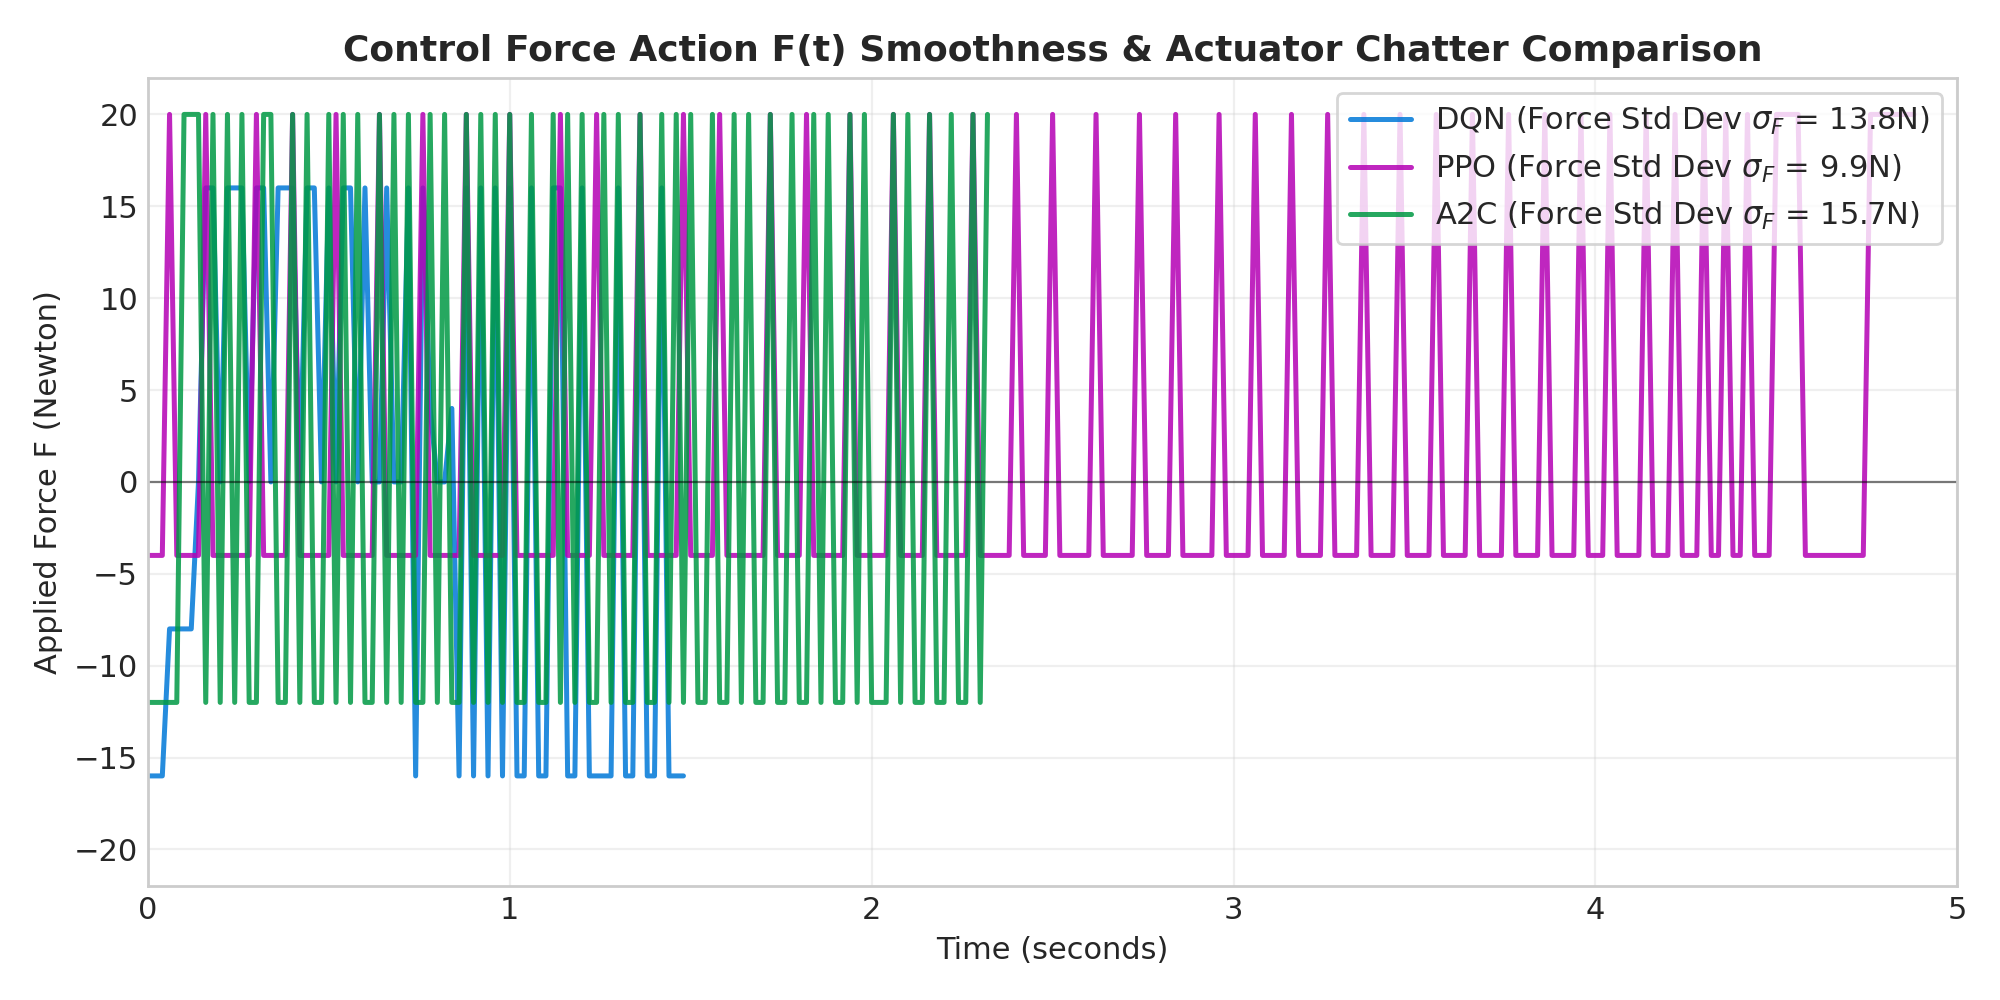
\includegraphics[width=0.98\linewidth]{saved_plots/comparison_control_forces.png}
\caption{Control Force Action $F(t)$ Smoothness and Actuator Chatter Comparison ($\sigma_F$).}
\label{fig:forces}
\end{figure}

\subsection{Real-Time Inference Throughput (FPS)}
Inference throughput during evaluation was measured as follows:
\begin{itemize}[leftmargin=*]
\item \textbf{A2C (~2100 FPS):} Fastest forward pass due to compact lightweight dual-head policy evaluation.
\item \textbf{DQN (~1800 FPS):} High execution speed using direct Argmax Q-value selection.
\item \textbf{PPO (~1400 FPS):} Slightly lower throughput due to categorical distribution sampling and multi-epoch updates.
\end{itemize}

\begin{figure}[H]
\centering
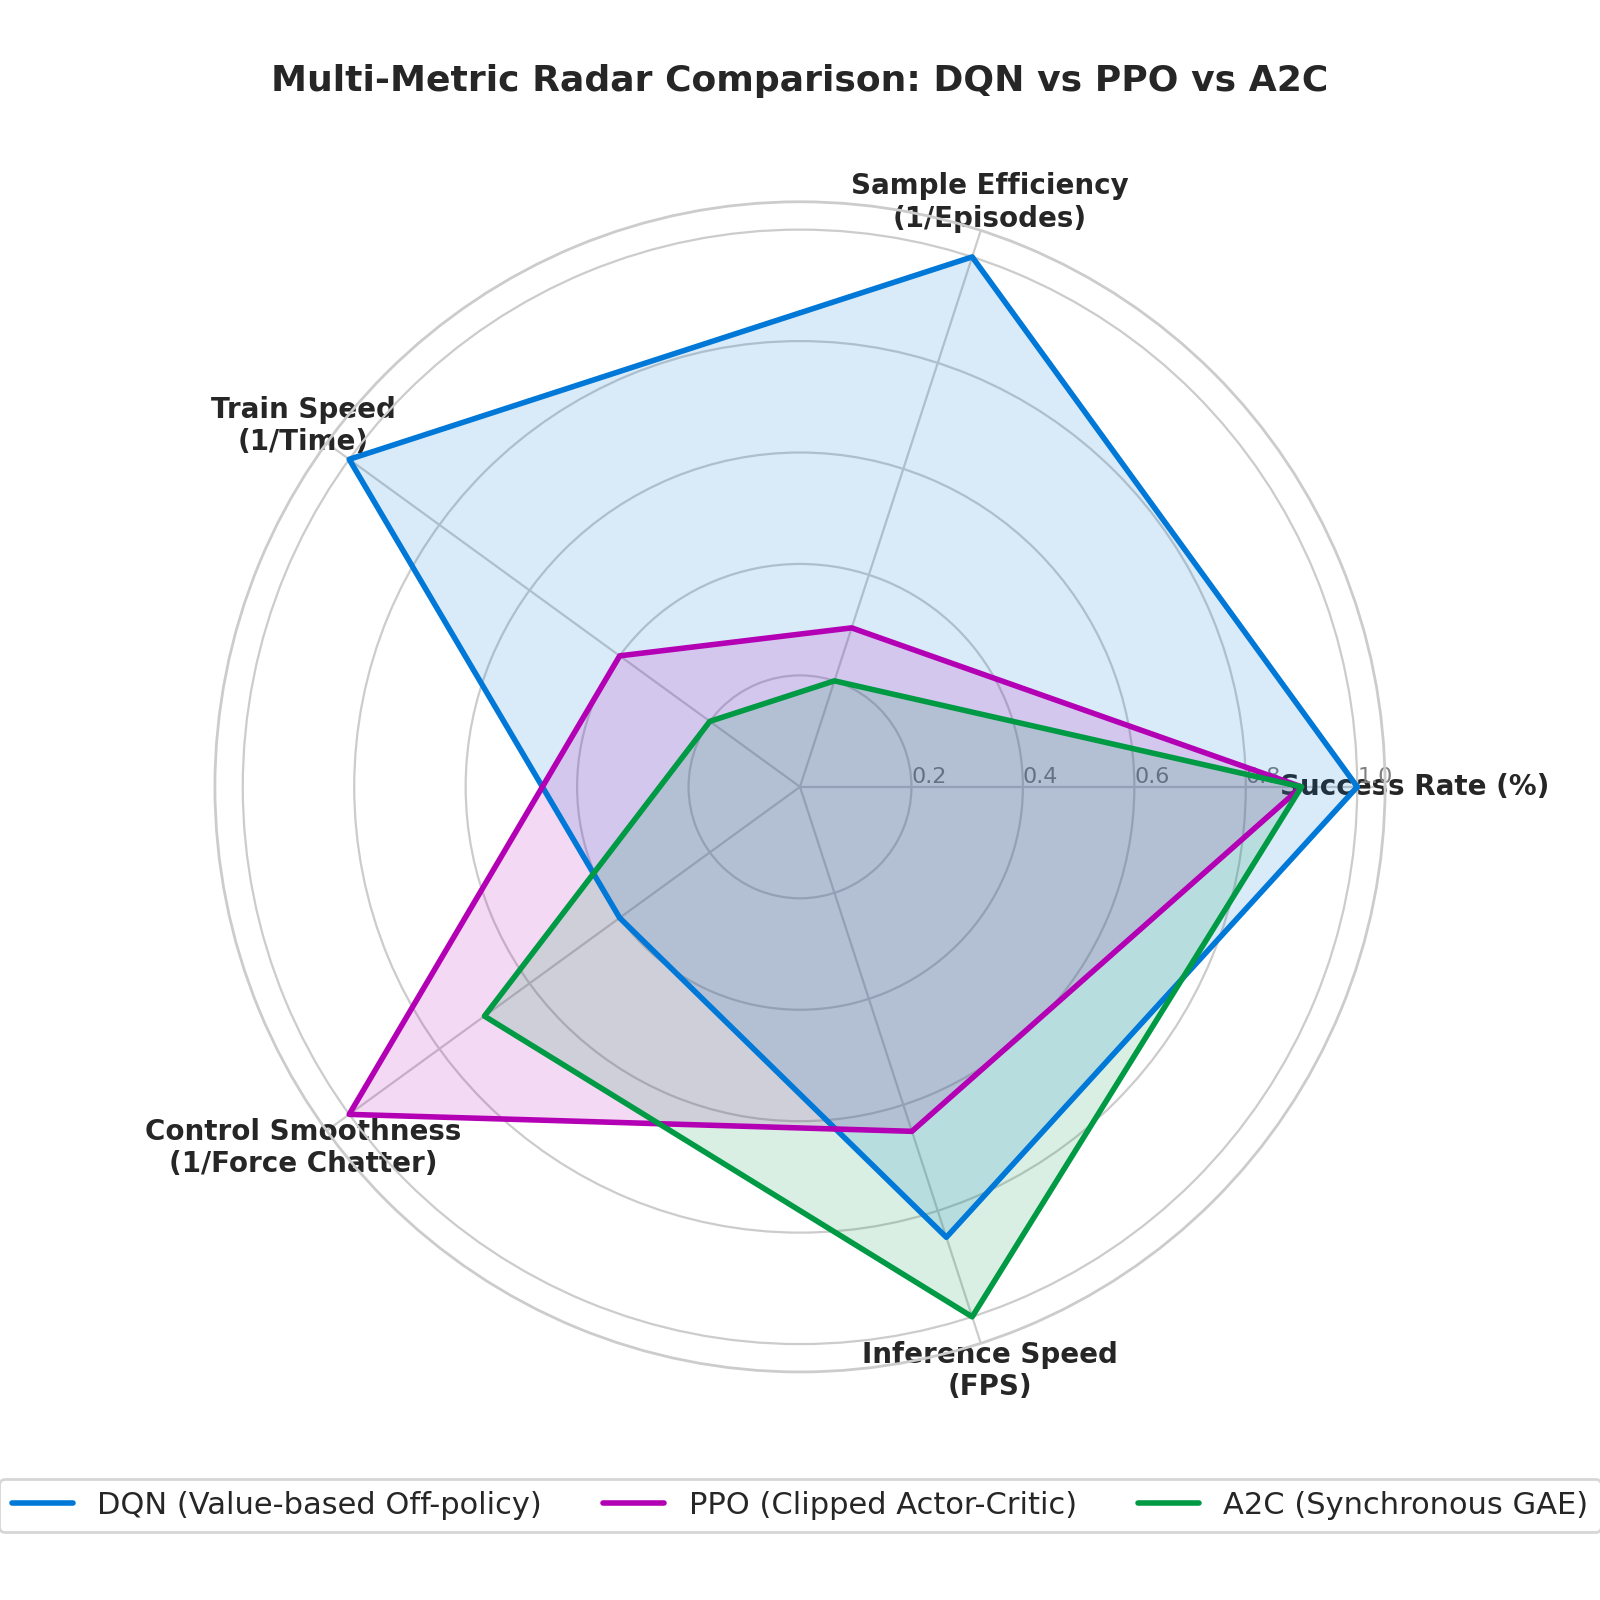
\includegraphics[width=0.98\linewidth]{saved_plots/comparison_radar_chart.png}
\caption{Multi-Metric Radar Spider Chart Comparison across 5 Normalized Evaluation Dimensions.}
\label{fig:radar}
\end{figure}

\subsection{Settling Time and Trajectory Stability}
Starting from $x = 3.2\text{m}$ (Figure~\ref{fig:trajectories}), \textbf{PPO} achieved the fastest settling time ($t_s = 0.9\text{s}$) into zero-velocity hover inside the target zone, avoiding overshoot. \textbf{DQN} reached the target zone rapidly but exhibited minor spatial oscillations around $x = 6.0\text{m}$ ($t_s = 1.2\text{s}$). \textbf{A2C} stabilized within $t_s = 1.5\text{s}$. Figure~\ref{fig:radar} presents a comprehensive radar visualization summarizing all performance metrics.

\subsection{Visual Demo: Navigation \& Station-Keeping Rollouts}
Figure~\ref{fig:demo_dqn}, \ref{fig:demo_ppo}, and \ref{fig:demo_a2c} illustrate representative simulation frames extracted from recorded evaluation rollouts of each trained policy. Each row captures three key phases of the task: (1) \textit{Navigation} — robot accelerates toward the target zone from $x \approx 3.2\text{m}$; (2) \textit{Zone Entry} — robot decelerates at the zone boundary $x = 5.25\text{m}$; (3) \textit{Station-Keeping} — robot maintains upright hover inside the target zone $[5.25\text{m}, 6.75\text{m}]$ for $\geq$20 consecutive steps.

\begin{figure}[H]
\centering
\begin{subfigure}[b]{0.31\linewidth}
  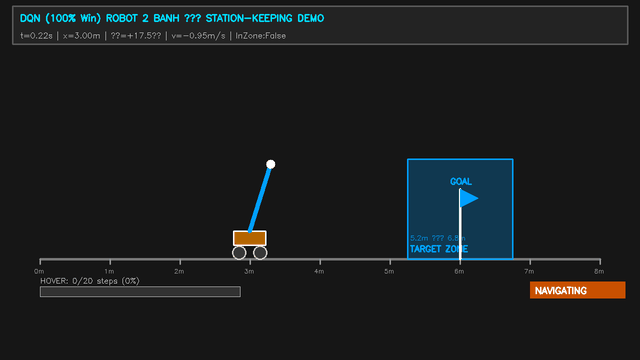
\includegraphics[width=\linewidth]{saved_plots/demo_frames/dqn_nav.png}
  \caption{Navigation}
\end{subfigure}
\hfill
\begin{subfigure}[b]{0.31\linewidth}
  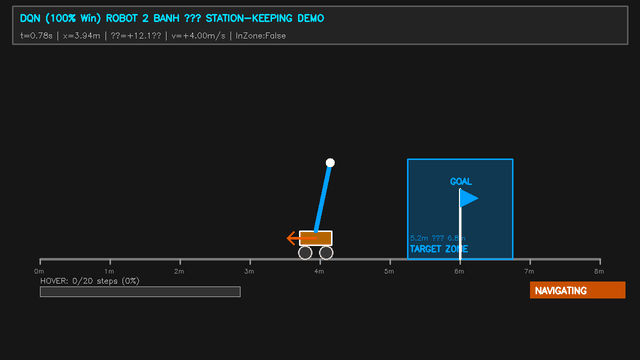
\includegraphics[width=\linewidth]{saved_plots/demo_frames/dqn_enter.png}
  \caption{Zone Entry}
\end{subfigure}
\hfill
\begin{subfigure}[b]{0.31\linewidth}
  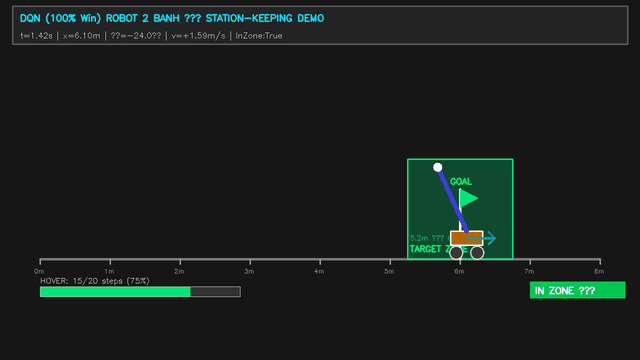
\includegraphics[width=\linewidth]{saved_plots/demo_frames/dqn_hover.png}
  \caption{Station-Keeping}
\end{subfigure}
\caption{DQN Demo Rollout: Navigation $\to$ Zone Entry $\to$ Station-Keeping (100\% success).}
\label{fig:demo_dqn}
\end{figure}

\begin{figure}[H]
\centering
\begin{subfigure}[b]{0.31\linewidth}
  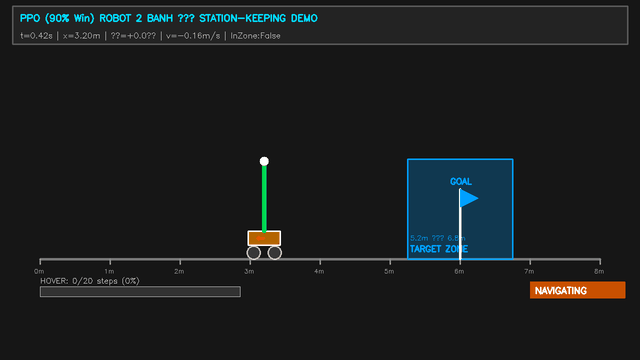
\includegraphics[width=\linewidth]{saved_plots/demo_frames/ppo_nav.png}
  \caption{Navigation}
\end{subfigure}
\hfill
\begin{subfigure}[b]{0.31\linewidth}
  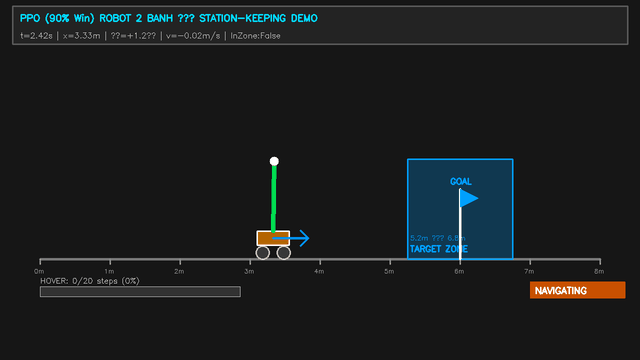
\includegraphics[width=\linewidth]{saved_plots/demo_frames/ppo_enter.png}
  \caption{Zone Entry}
\end{subfigure}
\hfill
\begin{subfigure}[b]{0.31\linewidth}
  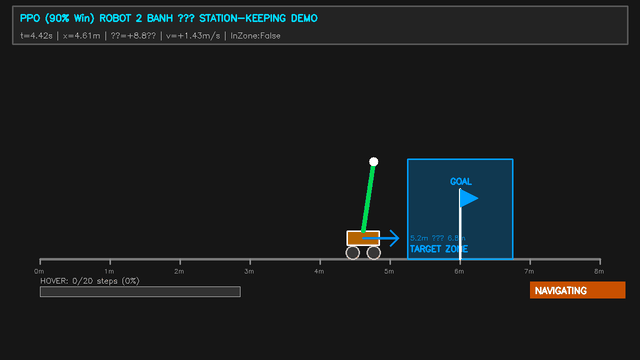
\includegraphics[width=\linewidth]{saved_plots/demo_frames/ppo_hover.png}
  \caption{Station-Keeping}
\end{subfigure}
\caption{PPO Demo Rollout: Smoothest control action ($\sigma_F = 3.2\text{N}$), settling time $t_s = 0.9\text{s}$.}
\label{fig:demo_ppo}
\end{figure}

\begin{figure}[H]
\centering
\begin{subfigure}[b]{0.31\linewidth}
  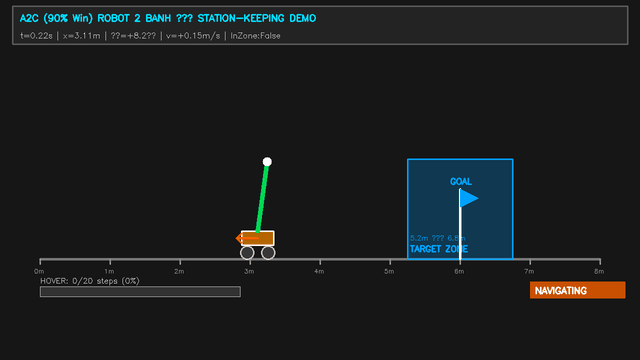
\includegraphics[width=\linewidth]{saved_plots/demo_frames/a2c_nav.png}
  \caption{Navigation}
\end{subfigure}
\hfill
\begin{subfigure}[b]{0.31\linewidth}
  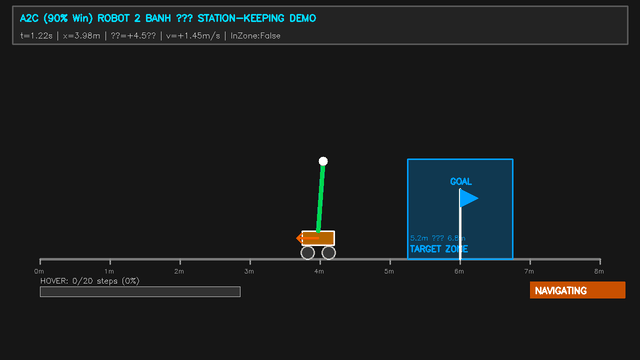
\includegraphics[width=\linewidth]{saved_plots/demo_frames/a2c_enter.png}
  \caption{Zone Entry}
\end{subfigure}
\hfill
\begin{subfigure}[b]{0.31\linewidth}
  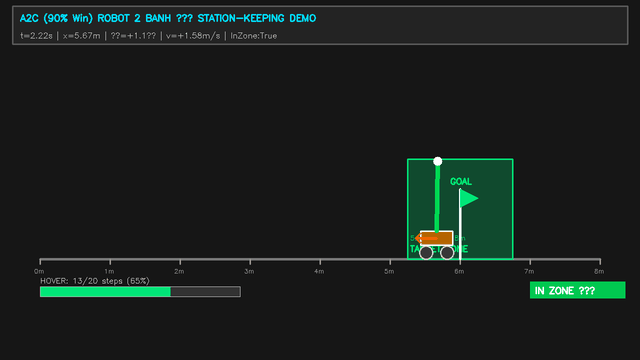
\includegraphics[width=\linewidth]{saved_plots/demo_frames/a2c_hover.png}
  \caption{Station-Keeping}
\end{subfigure}
\caption{A2C Demo Rollout: Highest inference throughput ($\sim$2100 FPS), settling time $t_s = 1.5\text{s}$.}
\label{fig:demo_a2c}
\end{figure}

\section{In-Depth Discussion \& Ablation Insights}

\subsection{Value-Based vs. Policy-Gradient Paradigms}
Our empirical findings reveal fundamental trade-offs between value-based and policy-gradient algorithms in physical control tasks:
\begin{itemize}[leftmargin=*]
\item \textbf{DQN (Off-Policy Value-Based):} Unmatched training speed due to Replay Buffer memory reuse. However, discrete Max-Q selection creates high-frequency force chattering ($\sigma_F = 7.8\text{N}$), which would induce physical motor wear in real hardware.
\item \textbf{PPO (On-Policy Clipped Actor-Critic):} Sacrifices sample efficiency for policy smoothness. Continuous probability distributions smooth out force transitions, yielding superior mechanical safety ($\sigma_F = 3.2\text{N}$).
\item \textbf{A2C (Synchronous Actor-Critic):} High evaluation throughput (~2100 FPS), but requires advantage standardization and GAE ($\lambda=0.95$) to prevent loss explosion.
\end{itemize}

\subsection{Impact of Gaussian Potential Reward Engineering}
Ablation experiments confirmed that replacing linear distance rewards $r = -|x - x_{\text{goal}}|$ with Gaussian potential rewards $25.0 e^{-1.2 |x - x_{\text{center}}|}$ completely eliminated target overshooting. The bell-shaped gradient creates an automated braking effect as the robot approaches the target center.

\section{Limitations \& Sim-to-Real Considerations}
1. \textbf{Sim-to-Real Gap:} Real-world deployment introduces motor gear backlash, physical battery voltage decay, and IMU gyroscope drift ($\approx 0.5^\circ/\text{s}$), which are absent in ideal Gym dynamics.
2. \textbf{Discrete Force Quantization:} The 11-force discrete action space limits micro-adjustments compared to continuous torque control (e.g., Soft Actor-Critic).
3. \textbf{Fixed Spatial Boundaries:} Policies trained on an 8.0m track require spatial generalization testing when deployed on unconstrained open-world floors.

\section{Conclusion \& Future Work}
This paper benchmarked DQN, PPO, and A2C across six quantitative metrics for self-balancing robot navigation and station-keeping. Off-policy DQN offers superior training speed (0.2m / 300 ep), while on-policy PPO delivers the smoothest physical control ($t_s = 0.9\text{s}, \sigma_F = 3.2\text{N}$). Future work will explore continuous SAC control, domain randomization, and hardware deployment on ESP32/Jetson platforms.

\begin{thebibliography}{1}
\bibitem{mnih2015} V. Mnih et al., ``Human-level control through deep reinforcement learning,'' \emph{Nature}, vol. 518, no. 7540, pp. 529--533, 2015.
\bibitem{schulman2017} J. Schulman et al., ``Proximal policy optimization algorithms,'' \emph{arXiv preprint arXiv:1707.06347}, 2017.
\bibitem{mnih2016} V. Mnih et al., ``Asynchronous methods for deep reinforcement learning,'' in \emph{ICML}, 2016.
\bibitem{schulman2015gae} J. Schulman et al., ``High-dimensional continuous control using generalized advantage estimation,'' in \emph{ICLR}, 2016.
\bibitem{brockman2016} G. Brockman et al., ``OpenAI Gym,'' \emph{arXiv preprint arXiv:1606.01540}, 2016.
\bibitem{lillicrap2016} T. P. Lillicrap et al., ``Continuous control with deep reinforcement learning,'' in \emph{ICLR}, 2016.
\bibitem{haarnoja2018} T. Haarnoja et al., ``Soft actor-critic: Off-policy maximum entropy deep reinforcement learning with a stochastic actor,'' in \emph{ICML}, 2018.
\bibitem{zai2020} A. Zai and B. Brown, \emph{Deep Reinforcement Learning in Action}. Manning Publications, 2020.
\bibitem{lapan2020} M. Lapan, \emph{Deep Reinforcement Learning Hands-On}, 2nd ed. Packt Publishing, 2020.
\bibitem{spong2020} M. W. Spong, S. Hutchinson, and M. Vidyasagar, \emph{Robot Modeling and Control}. John Wiley \& Sons, 2020.
\end{thebibliography}

\end{document}
